\section{Tecnologie}
Tecnologie adottate e motivazioni.

\subsection{MERN Stack}
La scelta tecnologica per questo progetto, dopo la fase di design dell'archittettura 
è ricatuta sullo stack \textbf{MERN}, acronimo di \textbf{MongoDB}, \textbf{Express}, \textbf{React}, \textbf{NodeJS}.

Questo significa che la RestApi è un'applicazione \textbf{NodeJS} che, 
grazie alla programmazione Asincrona in linguaggio JavaScript, 
la rende estermamente reattiva alle richieste degli utenti rispetto altre tecnologie server-side come PHP ed ASP. 
Inoltre la natura Single Thread del linguaggio ci ha alleggerito dal compito di gestire la concorrenza,
soprattutto in vista della gestione delle puntate delle aste che potrebbero avvenire da più utenti e molto ravvicinate prima della scandeza.

Il backend è supporto del pacchetto \textbf{Express}, 
un leggero e minimalista framework che mette a disposizione tutti gli strumenti necessari per una gestione delle richieste HTTP, 
così da pensare solo alla logica dell'applicazione.

I dati sono salvati su MongoDB, un database non relazionale molto reattivo ed adatto per veloci operazioni di Input/Output, 
altro tema molto importante per quanto riguarda le puntate dell'asta.

Dal momento che il FrontEnd è una SPA, la scelta poteva ricadere tra i tre framework più diffusi attualmente: React, Angular e Vue.
La scelta per questo progetto è stata \textbf{React}, una libreria JavaScript per creare SPA fortemente incentrata sui componenti, per i seguenti motivi:

\begin{itemize}
	\item Consideriamo Angular prolisso, genera una grande quantità di file come Java vincolando molto lo sviluppatore a rispettare la sua struttura. 
	Inoltre ha una curva di Apprendimento maggiore rispetto gli altri.
	\item Vue è una buona soluzione ma più giovane rispetto gli altri due framework e quindi attualmente ha meno supporto e pacchetti rispetto a React 
	(11M di download settimanali per React contro i 2M di Vue come da Figura \underline{\ref{fig:openbaseReact}} e \underline{\ref{fig:openbaseVue}}). 
	Questa è una considerazione importante da sviluppatore in quanto se ci si dovesse imbattere in qualche problema risulta più complesso trovare soluzioni online.
	\item A livello soggettivo apprezziamo maggiormente il metodo di lavoro di React. 
	\item Come da Figura \underline{\ref{fig:frameworks}} React continua ad essere molto apprezzato dalla comunity, anche a distanza di anni. 
\end{itemize} 

\begin{figure} 
	\centering
	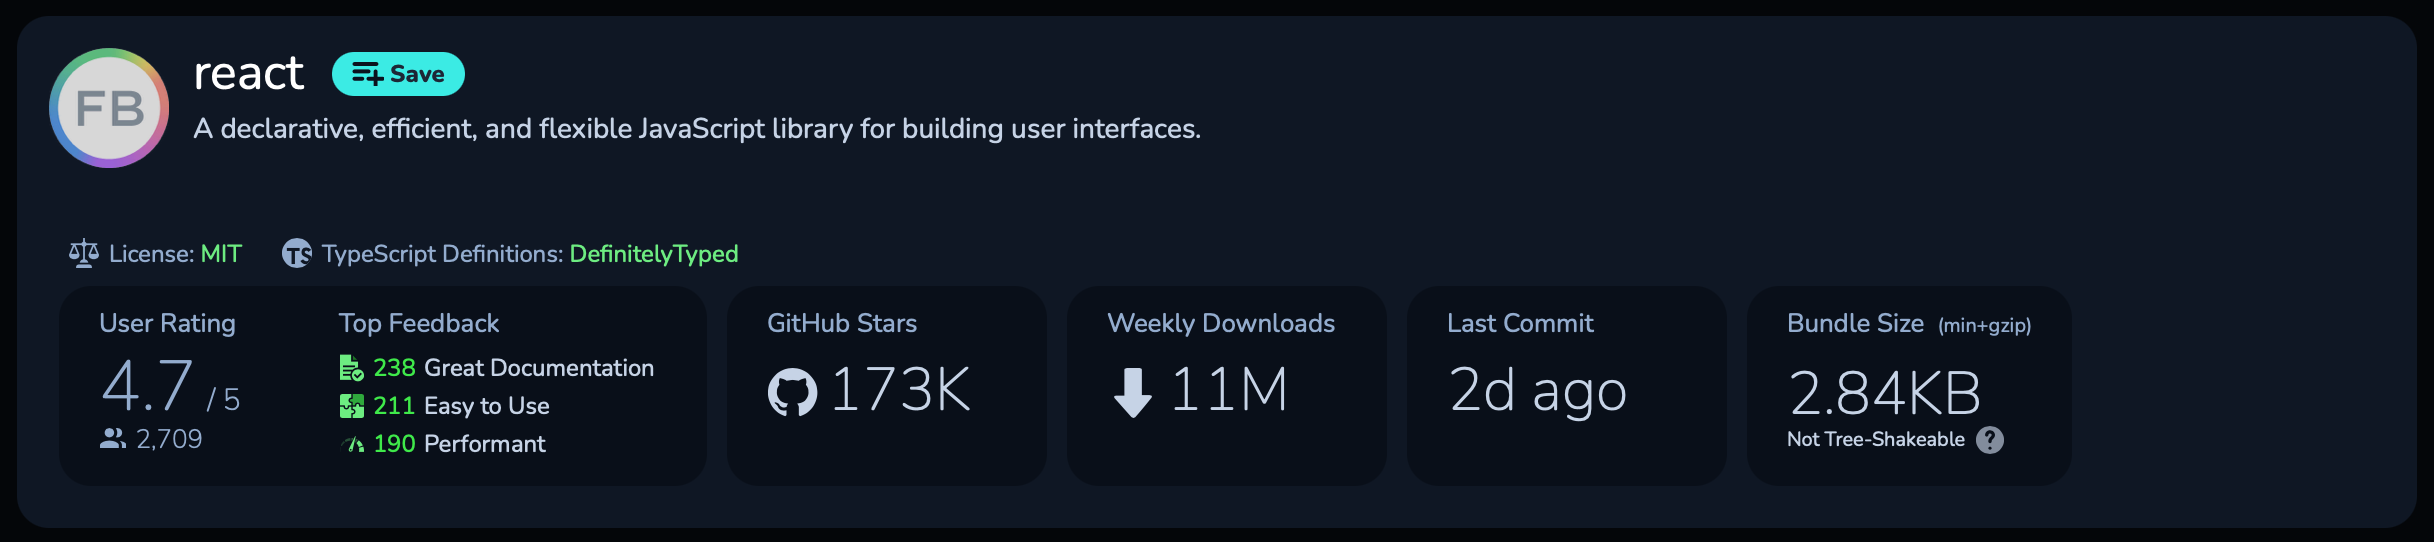
\includegraphics[width=\textwidth,keepaspectratio]{openbase-react.jpg}
	\caption{Statistiche React su \underline{\href{https://openbase.com/js/react}{openbase.com}}}
	\label{fig:openbaseReact}
\end{figure}
\begin{figure} 
	\centering
	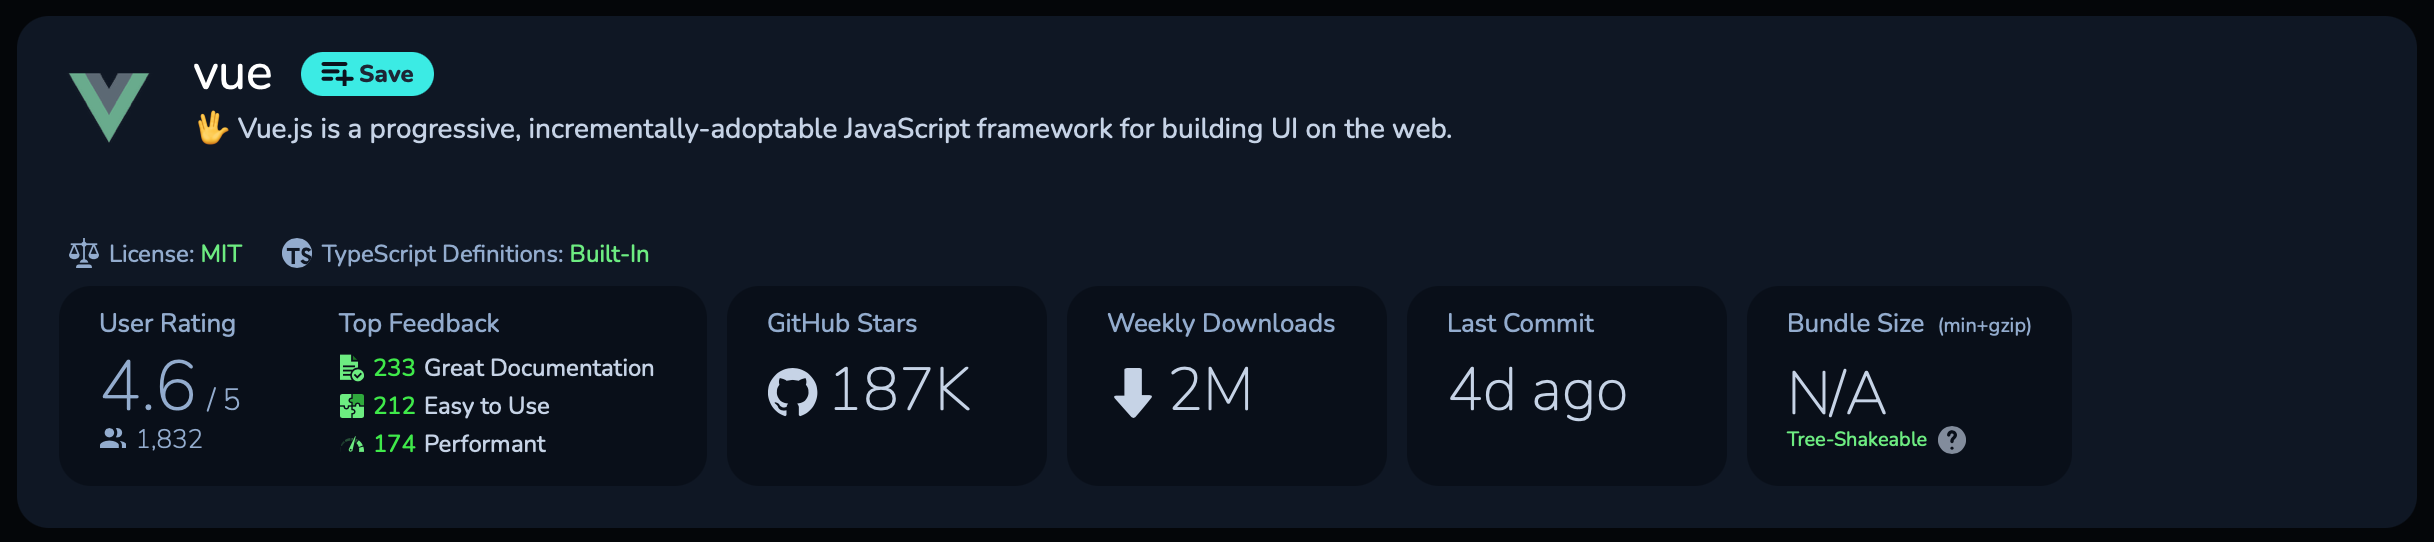
\includegraphics[width=\textwidth,keepaspectratio]{openbase-vue.jpg}
	\caption{Statistiche Vue su \underline{\href{https://openbase.com/js/vue}{openbase.com}}}
	\label{fig:openbaseVue}
\end{figure}
\begin{figure} 
	\centering
	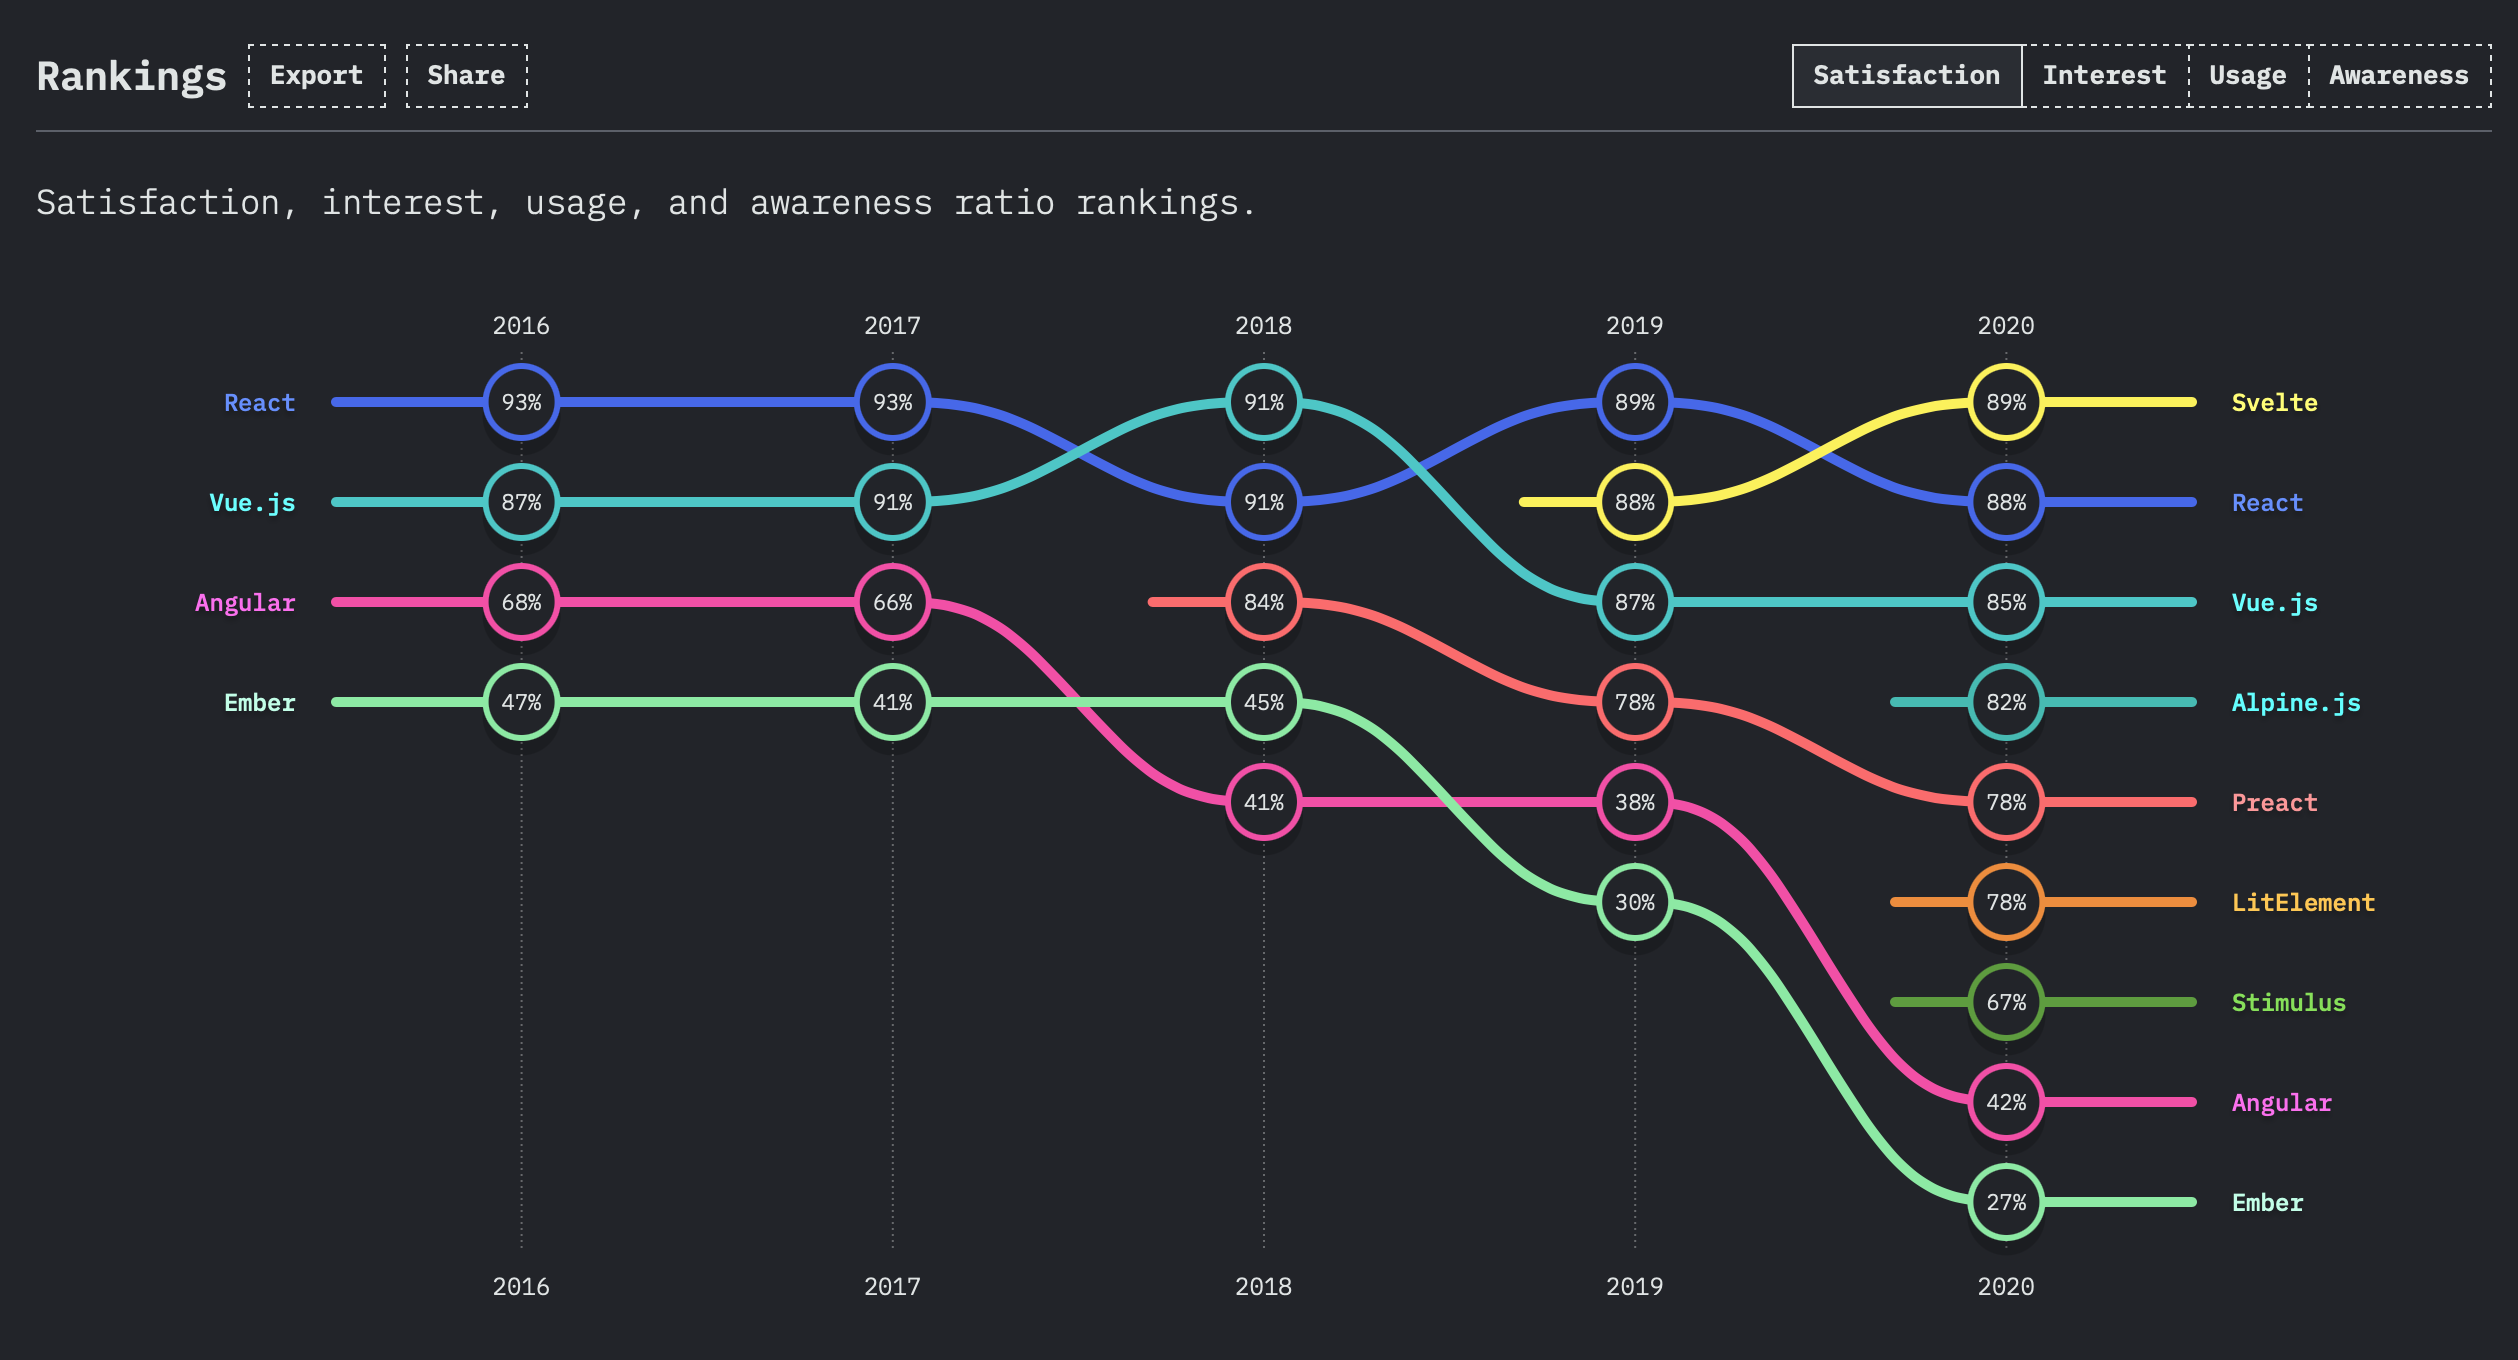
\includegraphics[width=\textwidth,keepaspectratio]{frameworks.jpg}
	\caption{Comparativa Framework \underline{\href{https://2020.stateofjs.com/en-US/technologies/front-end-frameworks/}{2020.stateofjs.com}}}
	\label{fig:frameworks}
\end{figure}

\clearpage

\subsection{Sviluppo}
Sviluppando in locale, abbiamo ricreato l'archittettura del sistema attraverso \textbf{Docker Compose}, 
ignorando la CDN in quanto non necessaria durante lo sviluppo.

Attraverso Docker Compose si sono costruiti i seguenti container:
\begin{itemize}
	\item \textbf{mongo}: database MongoDB versione 5.0.1-focal
	\item \textbf{api}: server contenente la RestApi in NodeJS
	\item \textbf{web}: server per la generazione del FrontEnd in React durante la fase di Sviluppo. In caso di Release sarà necessaria lanciare il comando build per generare tutti i file statici HTML, Javascript e CSS da caricare su S3
	\item \textbf{blockchain}: container generato ad hoc e pubblicato su DockerHub per lavorare con la blockchain EOS
	\item \textbf{localstack}: container per emulare i servizi di AWS (Amazon Web Services) del quale abbiamo utilizzato solo S3 per il caricamento delle immagini.
\end{itemize}

Lavorando su GitHub in team, si è deciso di utilizzare tutti \textbf{VScode} per scrivere codice, 
supportati dai pacchetti \textbf{\underline{\href{https://eslint.org/docs/user-guide/getting-started}{ESlint}}} e \textbf{\underline{\href{https://prettier.io/docs/en/index.html}{Prettier}}} per permetterci di formattare allo stesso modo il codice
e guidarci nelle "best practice" della programmazione secondo l'estensione di  \textbf{\underline{\href{https://www.npmjs.com/package/eslint-config-airbnb}{AirBnb}}}.
 
\subsection{BackEnd}
Pacchetti utilizzati a supporto per lo sviluppo della RestApi:

\begin{itemize}
	\item \textbf{\underline{\href{https://ajv.js.org/}{ajv}}}: validazione tramite JSON schema dei parametri e body inviati tramite le richieste alla RestApi
	\item \textbf{\underline{\href{https://www.npmjs.com/package/aws-sdk}{aws-sdk}}}: necessaria per interagire con S3 per il salvataggio delle immagini
	\item \textbf{\underline{\href{https://www.npmjs.com/package/bcryptjs}{bcryptjs}}}: libreria di criptazione utilizzata per salvare la password sul database
	\item \textbf{\underline{\href{http://expressjs.com/en/resources/middleware/cookie-parser.html}{cookie-parser}}}: estensione di express per poter agevolmente estrarre i cookie dalle richieste, utile per l'autenticazione.
	\item \textbf{\underline{\href{https://www.npmjs.com/package/cors}{cors}}}: estensione di express per gestire il Cross-Origin Resource Sharing e proteggere la RestApi
	\item \textbf{\underline{\href{https://www.npmjs.com/package/crypto-js}{crypto-js}}}: libreria di criptazione utilizzata per le chiavi pubbliche su blockchain
	\item \textbf{\underline{\href{https://ejs.co/}{ejs}}}: linguaggio embedded javascript per la generazione di template html di email
	\item \textbf{\underline{\href{https://www.npmjs.com/package/email-templates}{email-templates}}}: gestione dei template delle email
	\item \textbf{\underline{\href{https://www.npmjs.com/package/eosjs}{eosjs}}}: libreria per comunicare con la blockchain 
	\item \textbf{\underline{\href{https://jwt.io}{jsonwebtoken}}}: generazione e validazione di JSON Web Token utilizzati per l'autenticazione
	\item \textbf{\underline{\href{https://momentjs.com}{moment}}}: libreria per la gestione delle date
	\item \textbf{\underline{\href{https://mongoosejs.com}{mongoose}}}: object modelling per il database MongoDB
	\item \textbf{\underline{\href{https://nodemailer.com/about}{nodemailer}}}: libreria per l'invio delle email
	\item \textbf{\underline{\href{http://www.passportjs.org}{passport}}}: middleware per l'implementazione di vari sistemi di autenticazione dei quali abbiamo utilizzato "passport-local" per il login con credenziali salvate su database e "passport-jwt" per la validazione del JSON Web Token
	\item \textbf{\underline{\href{https://socket.io/}{socket.io}}}: socket server per la comunicazione in tempo reale utilizzato per le puntate
	\item \textbf{\underline{\href{https://www.npmjs.com/package/sprintf-js}{sprintf-js}}}: utility per aggiungere la funzionalità sprintf a NodeJs
	\item \textbf{\underline{\href{https://www.npmjs.com/package/uuid}{uuid}}}: libreria di generazione chiavi con standar uuid, utilizzata per la generazione dei refresh token
\end{itemize}

Al fine di testare le email inviate dalla RestApi, abbiamo utilizzato il servizio \textbf{\underline{\href{https://mailtrap.io}{MailTrap}}}
che intercetta tutte le email inviate e le mostra in una casella di posta 
dove abbiamo potuto verificare la corretta visualizzazione sui vari dispositivi 
ed eventuali errori di compatibilità tra client (Firure \underline{\ref{fig:mailtrapValid}} e \underline{\ref{fig:mailtrap}}).

Per quanto riguarda i test realizzati sul BackEnd si è deciso di optare per il paccheto \textbf{\underline{\href{https://jestjs.io/docs/getting-started}{Jest}}},
supportato da \textbf{\underline{\href{https://www.npmjs.com/package/supertest}{Supertest}}} e \textbf{\underline{\href{https://github.com/nodkz/mongodb-memory-server}{Mongodb-memory-server}}}.
Supertest è un pacchetto utile per testare le chiamate ad una RestApi mentre 
Mongodb-memory-server permette di virtualizzare in memoria il database durante la fase di test direttamente, 
evitando così di effettuare i test nel database presente sul container docker utilizzato da noi sviluppatori 
per provare l'applicativo in locale ed inizializzato tramite seed. 

\begin{figure}[H]
	\centering
	
\includegraphics[width=\textwidth,keepaspectratio]{mailtrap.png}
	\caption{Visualizzazione email su MailTrap}
	\label{fig:mailtrap}
\end{figure}

\begin{figure}[H]
	\centering
	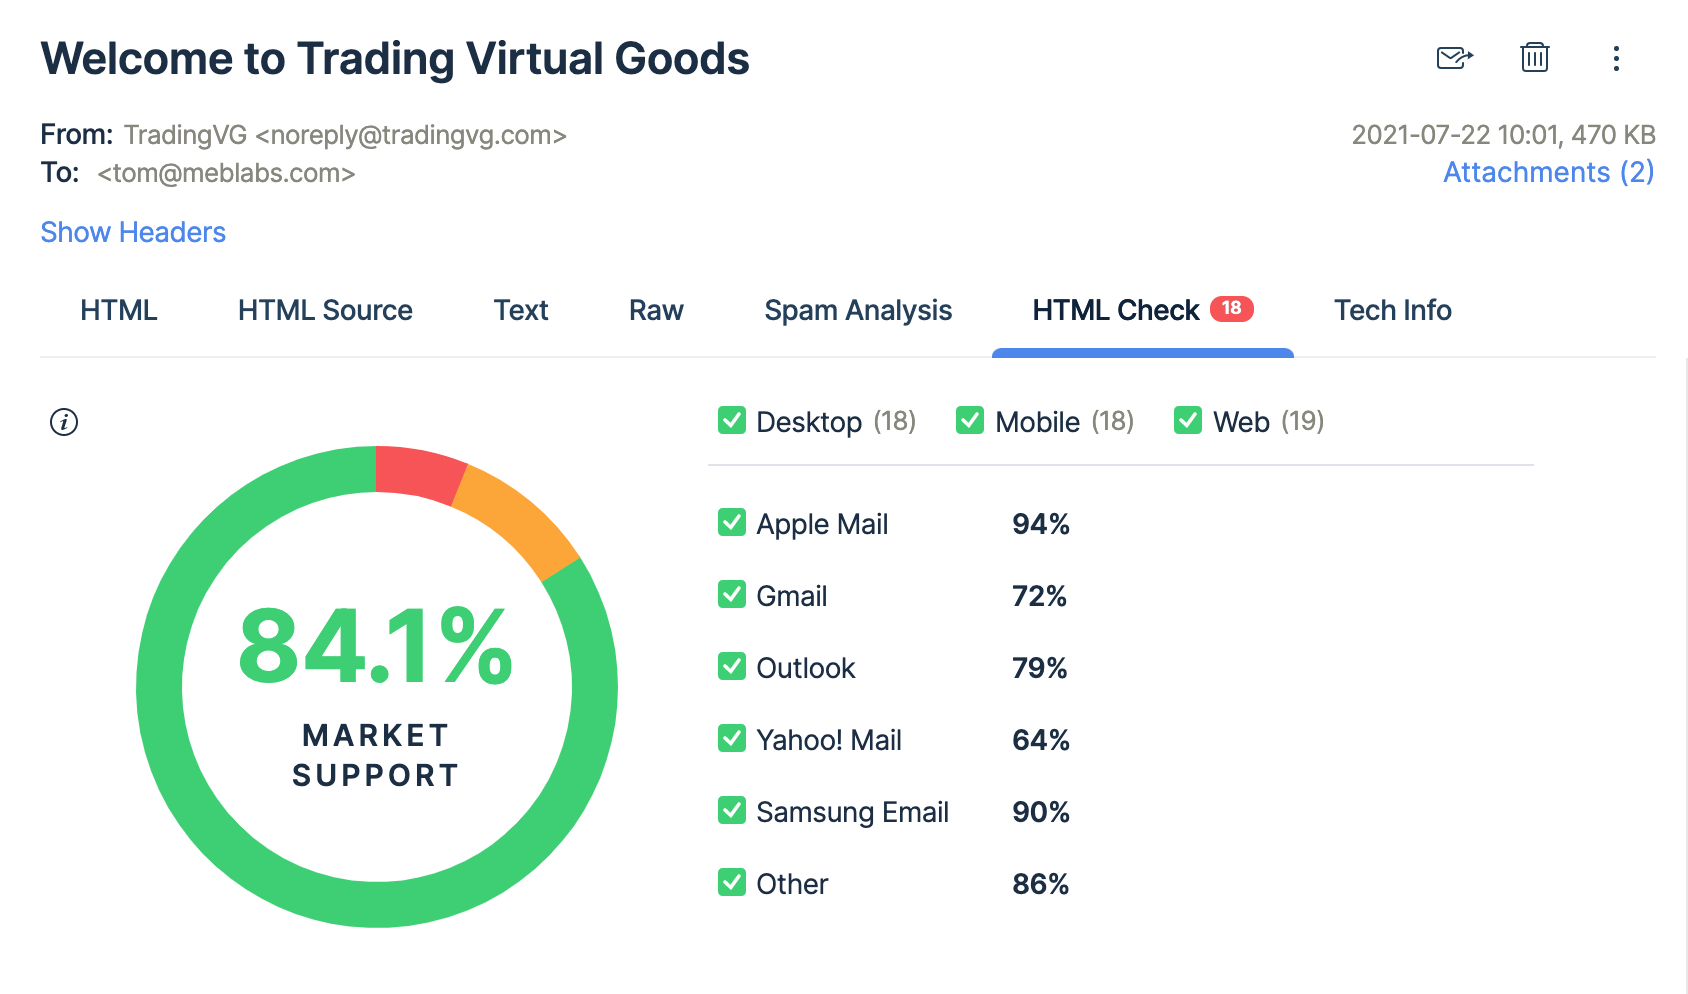
\includegraphics[width=\textwidth,keepaspectratio]{mailtrap-valid.jpg}
	\caption{Compatibilità email su MailTrap}
	\label{fig:mailtrapValid}
\end{figure}

\clearpage

\subsection{FrontEnd}
Il progetto del FrontEnd è stato creato con \textbf{\underline{\href{https://create-react-app.dev/}{Create React App}}}.

Pacchetti utilizzati a supporto del FrontEnd:

\begin{itemize}
	\item \textbf{\underline{\href{https://ant.design/}{ant}}}: componenti della User Interface
	\item \textbf{\underline{\href{https://www.npmjs.com/package/aws-sdk}{aws-sdk}}}: necessaria per interagire con S3 per il salvataggio delle immagini
	\item \textbf{\underline{\href{https://www.npmjs.com/package/axios}{axios}}}: per gestire le chiamate HTTP alla RestApi
	\item \textbf{\underline{\href{https://ant.design/docs/react/use-with-create-react-app}{craco}}}: plugin della Create React App per permettere l'utilizzo di LESS come transpiler dei CSS (Non abbiamo utilizzato SCSS perchè Ant è basato su LESS)
	\item \textbf{\underline{\href{https://react.i18next.com/latest/using-with-hooks}{i18next}}}: libreria per la gestione del multilingua e che fornisce un apposito Hook per React (useTranslation)
	\item \textbf{\underline{\href{https://momentjs.com}{moment}}}: libreria gestione delle tate
	\item \textbf{\underline{\href{https://reactrouter.com/web/guides/quick-start}{react-router-dom}}}: plugin di React per la gestione dei link
	\item \textbf{\underline{\href{https://www.npmjs.com/package/socket.io-client}{socket.io-client}}}: socket client per la comunicazione in tempo reale utilizzato per le puntate
	\item \textbf{\underline{\href{https://www.npmjs.com/package/sprintf-js}{sprintf-js}}}: utility per aggiungere la funzionalità sprintf a NodeJs
\end{itemize}

\clearpage

\subsection{EOS Blockchain}
La blockchain che abbiamo scelto è \textbf{\underline{\href{https://eos.io/}{EOS}}} in quanto: 

\begin{itemize}
	\item permette di scaricare i costi di transazioni/mantenimento direttamente sulla piattaforma TVG anzichè sugli artisti/utilizzatori
	\item è possibile interfacciarsi facilmente con Javascript
	\item è sufficientemente diffusa, anche se meno famosa dell'alternativa Ethereum
	\item è molto efficiente e veloce - è possibile eseguire una transazione in appena mezzo secondo contro svariati minuti delle altre alternative
	\item è green: il meccanismo del consenso distribuito è Delegated Proof of Stake che, contrariamente al Proof Of Work di Ethereum e Bitcoin, non richiede per funzionare l'impiego di alcuna computazione la quale attualmente porta i miners delle altre blockchain a competere con un dispendio energetico elevatissimo su scala mondiale
\end{itemize}

Al fine di fornire il servizio di creazione e trasferimento NFT occorre sviluppare uno Smart Contract, questo non è altro che un programma che viene eseguito dalla blockchain.
Abbiamo programmato lo Smart Conctract per EOS in \textbf{C++} utilizzando a supporto le seguenti librerie:

\begin{itemize}
	\item \textbf{\underline{\href{https://developers.eos.io/welcome/latest/getting-started-guide/local-development-environment/installing-eosiocdt}{eosio-cdt}}}: contract development toolkit
	\item \textbf{\underline{\href{https://www.boost.org/}{boost}}}: libreria per utilizzare tabelle di dati indicizzati in RAM
\end{itemize}